\section{Задание 2. Аппроксимация эллиптическим параболоидом}

\subsection{Постановка задачи}

Используя те же данные варианта 7 (см. таблицу~\ref{tab:data}), выполнить аппроксимацию функции двух переменных с помощью эллиптического параболоида. Требуется:
\begin{itemize}
    \item реализовать модель на языке Python;
    \item минимизировать MSE функцию потерь;
    \item построить кривую обучения (loss как функция от номера итерации);
    \item вычислить невязки на каждом объекте;
    \item построить модельную поверхность и линии уровня вместе с точками данных;
    \item записать аналитический вид модели.
\end{itemize}

\subsection{Математическая модель}

Эллиптический параболоид (общее уравнение второго порядка):

\begin{equation}\label{eq:paraboloid}
    z(x, y) = z_0 + a(x - x_0)^2 + b(y - y_0)^2 + 2h(x - x_0)(y - y_0),
\end{equation}

где $(x_0, y_0, z_0)$ --- координаты вершины; $a, b$ --- кривизны по осям $x$ и $y$; $h$ --- коэффициент смешанного члена. Условие эллиптичности: $ab > h^2$. Для пика (колоколообразной функции) необходимо $a < 0$, $b < 0$.

Вектор параметров: $\mathbf{p} = (z_0, x_0, y_0, a, b, h)$.

\subsection{Метод оптимизации}

Функция потерь --- MSE:
\begin{equation}
    L(\mathbf{p}) = \frac{1}{N}\sum_{i=1}^{N}\left(z(x_i, y_i; \mathbf{p}) - z_i\right)^2.
\end{equation}

Метод: \textbf{L-BFGS-B} с ограничениями:
\begin{itemize}
    \item $z_0 \in [-1, 10]$, $x_0, y_0 \in [0, 6]$;
    \item $a, b \in [-5, -0.01]$ (отрицательные для пика);
    \item $h \in [-2, 2]$.
\end{itemize}

Начальное приближение: вершина в точке максимума $z$, $a_0 = b_0 = -1.0$, $h_0 = 0$.

\subsection{Кривая обучения}

\begin{figure}[H]
    \centering
    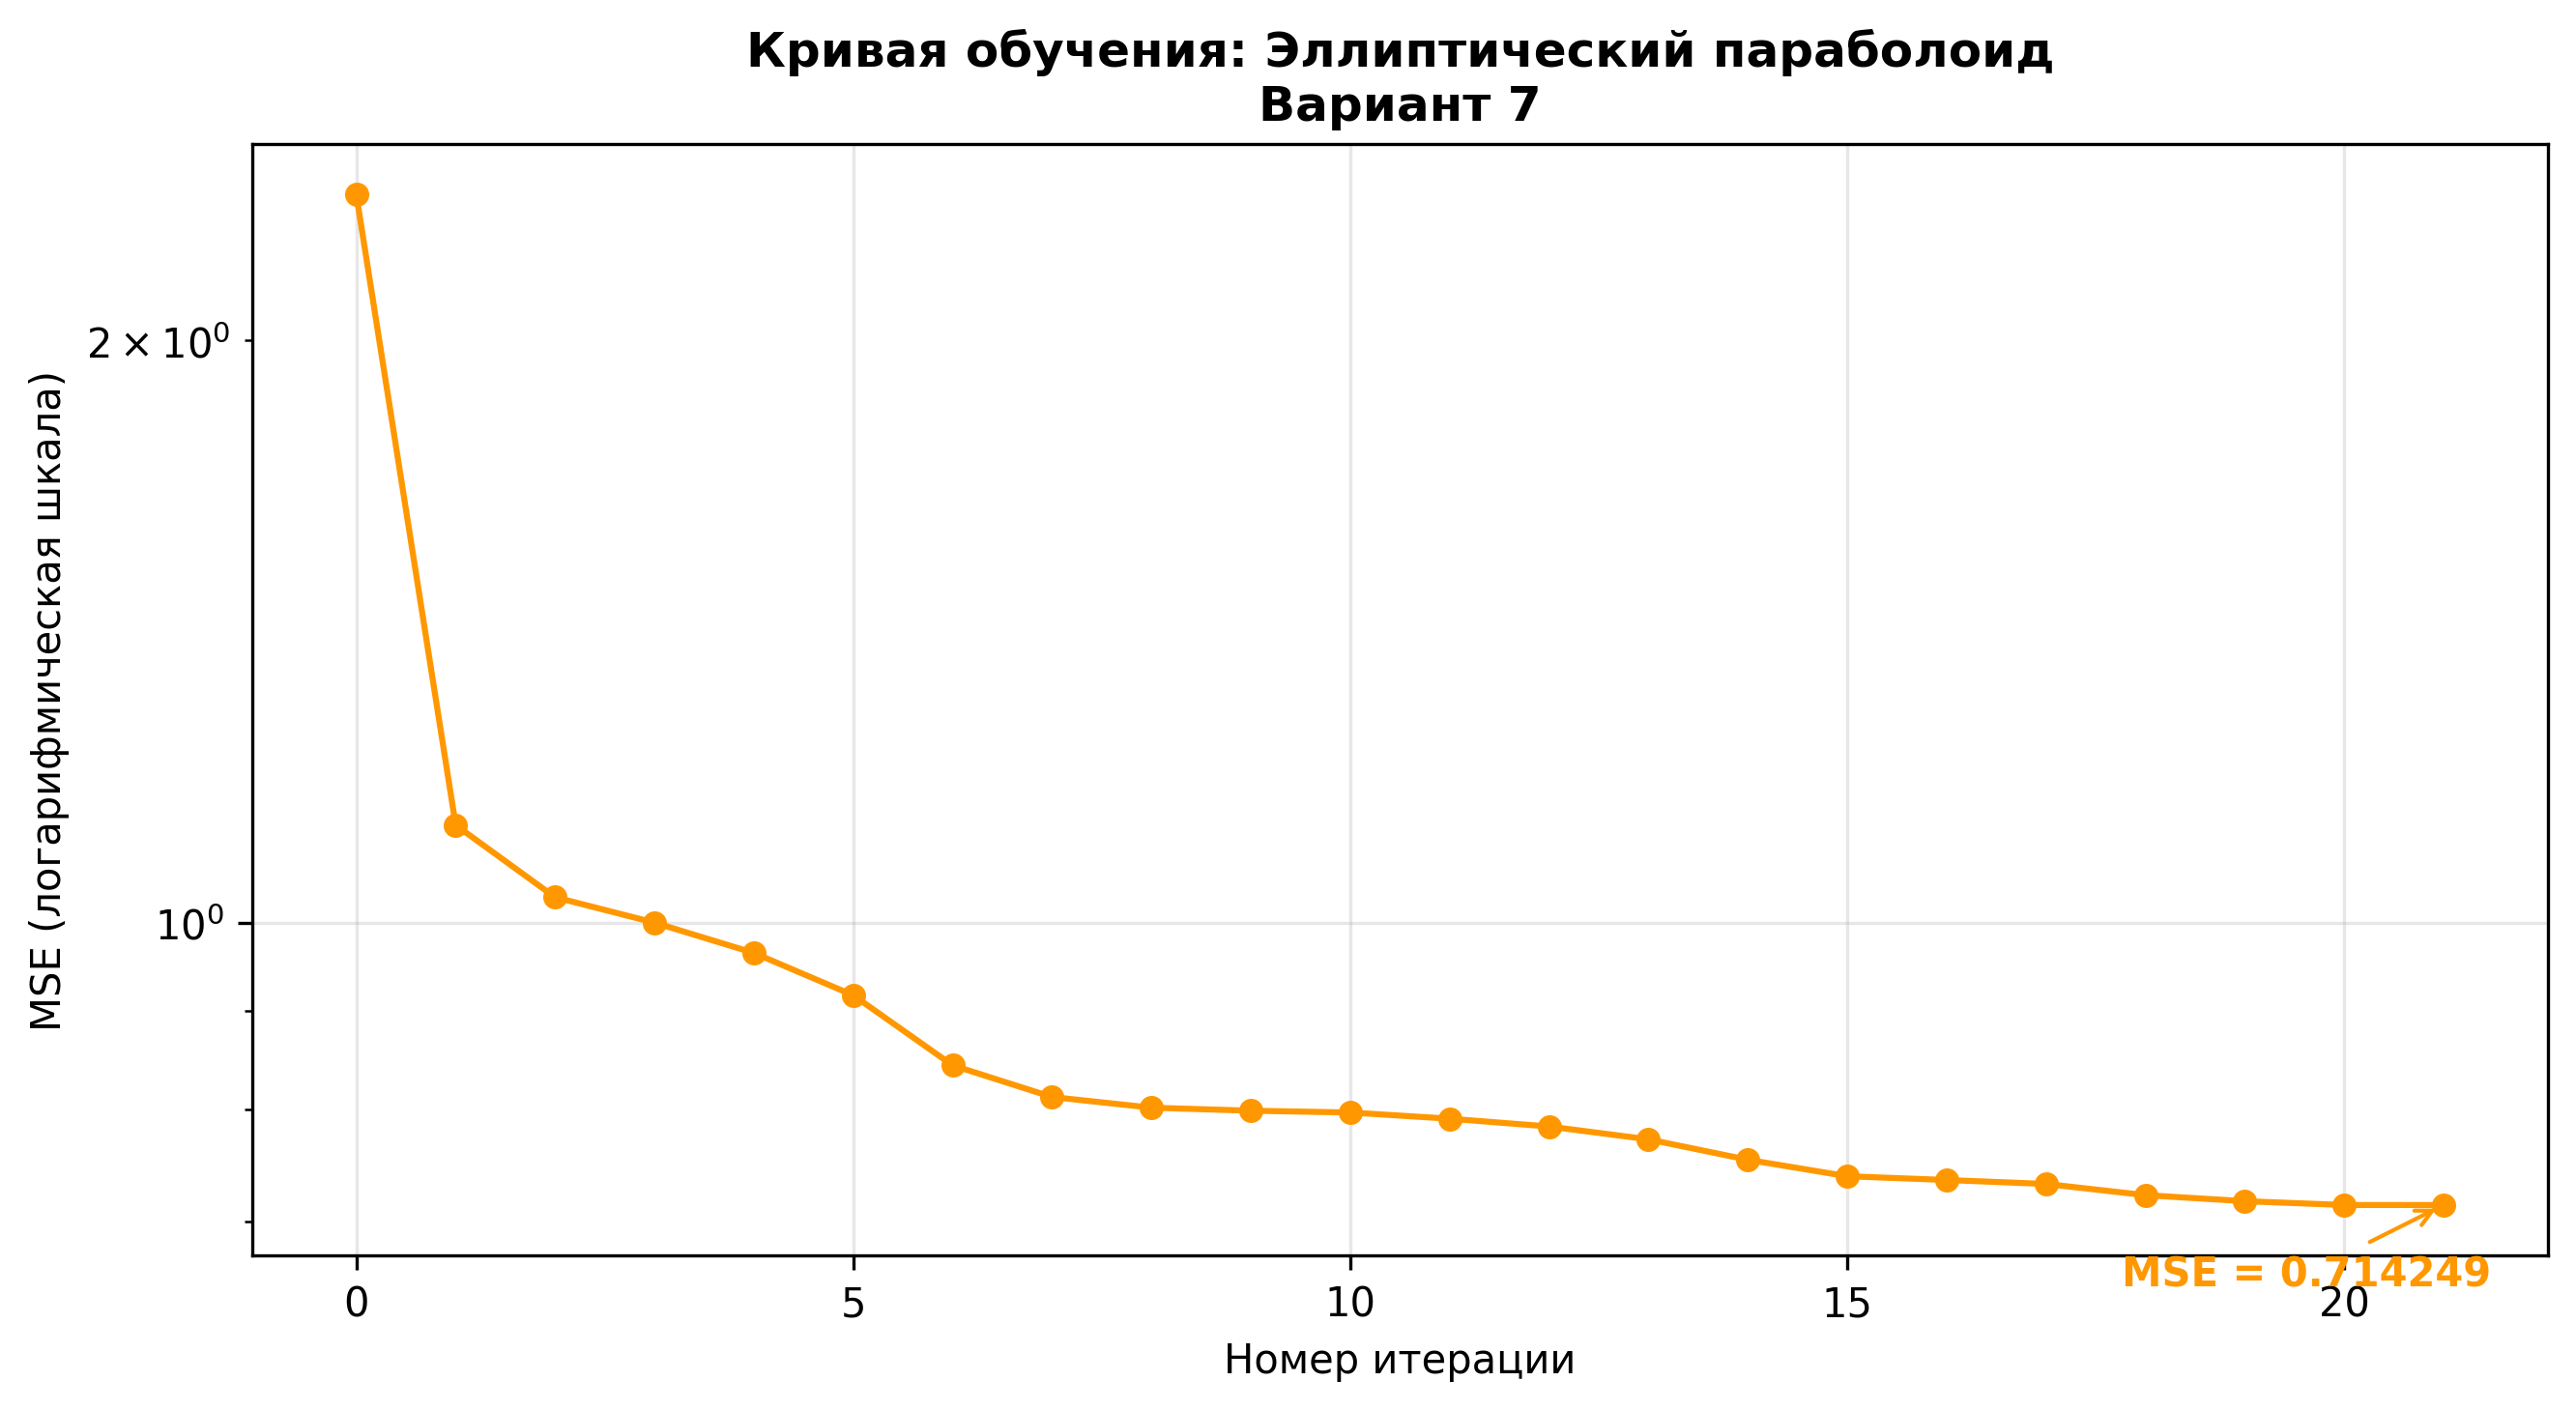
\includegraphics[width=0.85\textwidth]{pic/paraboloid_learning_curve.png}
    \caption{Кривая обучения эллиптического параболоида}
    \label{fig:parab_learning}
\end{figure}

На рис.~\ref{fig:parab_learning} показана динамика MSE в процессе оптимизации. Алгоритм сошёлся за 22 итерации. Конечное значение MSE = 0.7142. Лосс быстро убывает в первых итерациях, после 5-й итерации скорость сходимости замедляется.

\subsection{Результаты}

\begin{table}[H]
    \centering
    \caption{Оптимальные параметры параболоида}
    \label{tab:parab_params}
    \begin{tabular}{|c|c|}
        \hline
        \textbf{Параметр} & \textbf{Значение} \\
        \hline
        $z_0$ & 4.4065 \\
        $x_0$ & 3.4644 \\
        $y_0$ & 3.9737 \\
        $a$ & -1.5978 \\
        $b$ & -0.0962 \\
        $h$ & 0.3639 \\
        \hline
        Число итераций & 22 \\
        \hline
    \end{tabular}
\end{table}

\subsection{Аналитический вид модели}

\begin{equation}\label{eq:parab_result}
    \begin{aligned}
        z(x,y) = 4.4065 &- 1.5978 \cdot (x - 3.4644)^2 \\
                         &- 0.0962 \cdot (y - 3.9737)^2 \\
                         &+ 2 \cdot 0.3639 \cdot (x - 3.4644)(y - 3.9737).
    \end{aligned}
\end{equation}

\subsection{Таблица невязок}

\begin{table}[H]
    \centering
    \caption{Невязки эллиптического параболоида}
    \label{tab:parab_residuals}
    \begin{tabular}{|c|c|c|c|c|c|}
        \hline
        \textbf{Точка} & \textbf{$x$} & \textbf{$y$} & \textbf{$z_{факт}$} & \textbf{$z_{модель}$} & \textbf{Невязка} & \textbf{Кв. невязки} \\
        \hline
        0 & 1.10 & 1.10 & 0.29 & -0.3753 & -0.6653 & 0.4427 \\
        1 & 2.01 & 1.98 & 1.24 & 2.7546 & 1.5146 & 2.2939 \\
        2 & 3.01 & 2.85 & 4.94 & 4.3267 & -0.6133 & 0.3762 \\
        3 & 3.86 & 3.99 & 4.72 & 4.1611 & -0.5589 & 0.3123 \\
        4 & 5.10 & 4.90 & 0.77 & 1.1524 & 0.3824 & 0.1462 \\
        \hline
    \end{tabular}
\end{table}

MSE $= 0.7142$, RMSE $= 0.8451$. Наибольшая невязка наблюдается в точке 1 ($\pm 1.51$), наименьшая --- в точке 4 ($\pm 0.38$).

\subsection{Визуализация}

\begin{figure}[H]
    \centering
    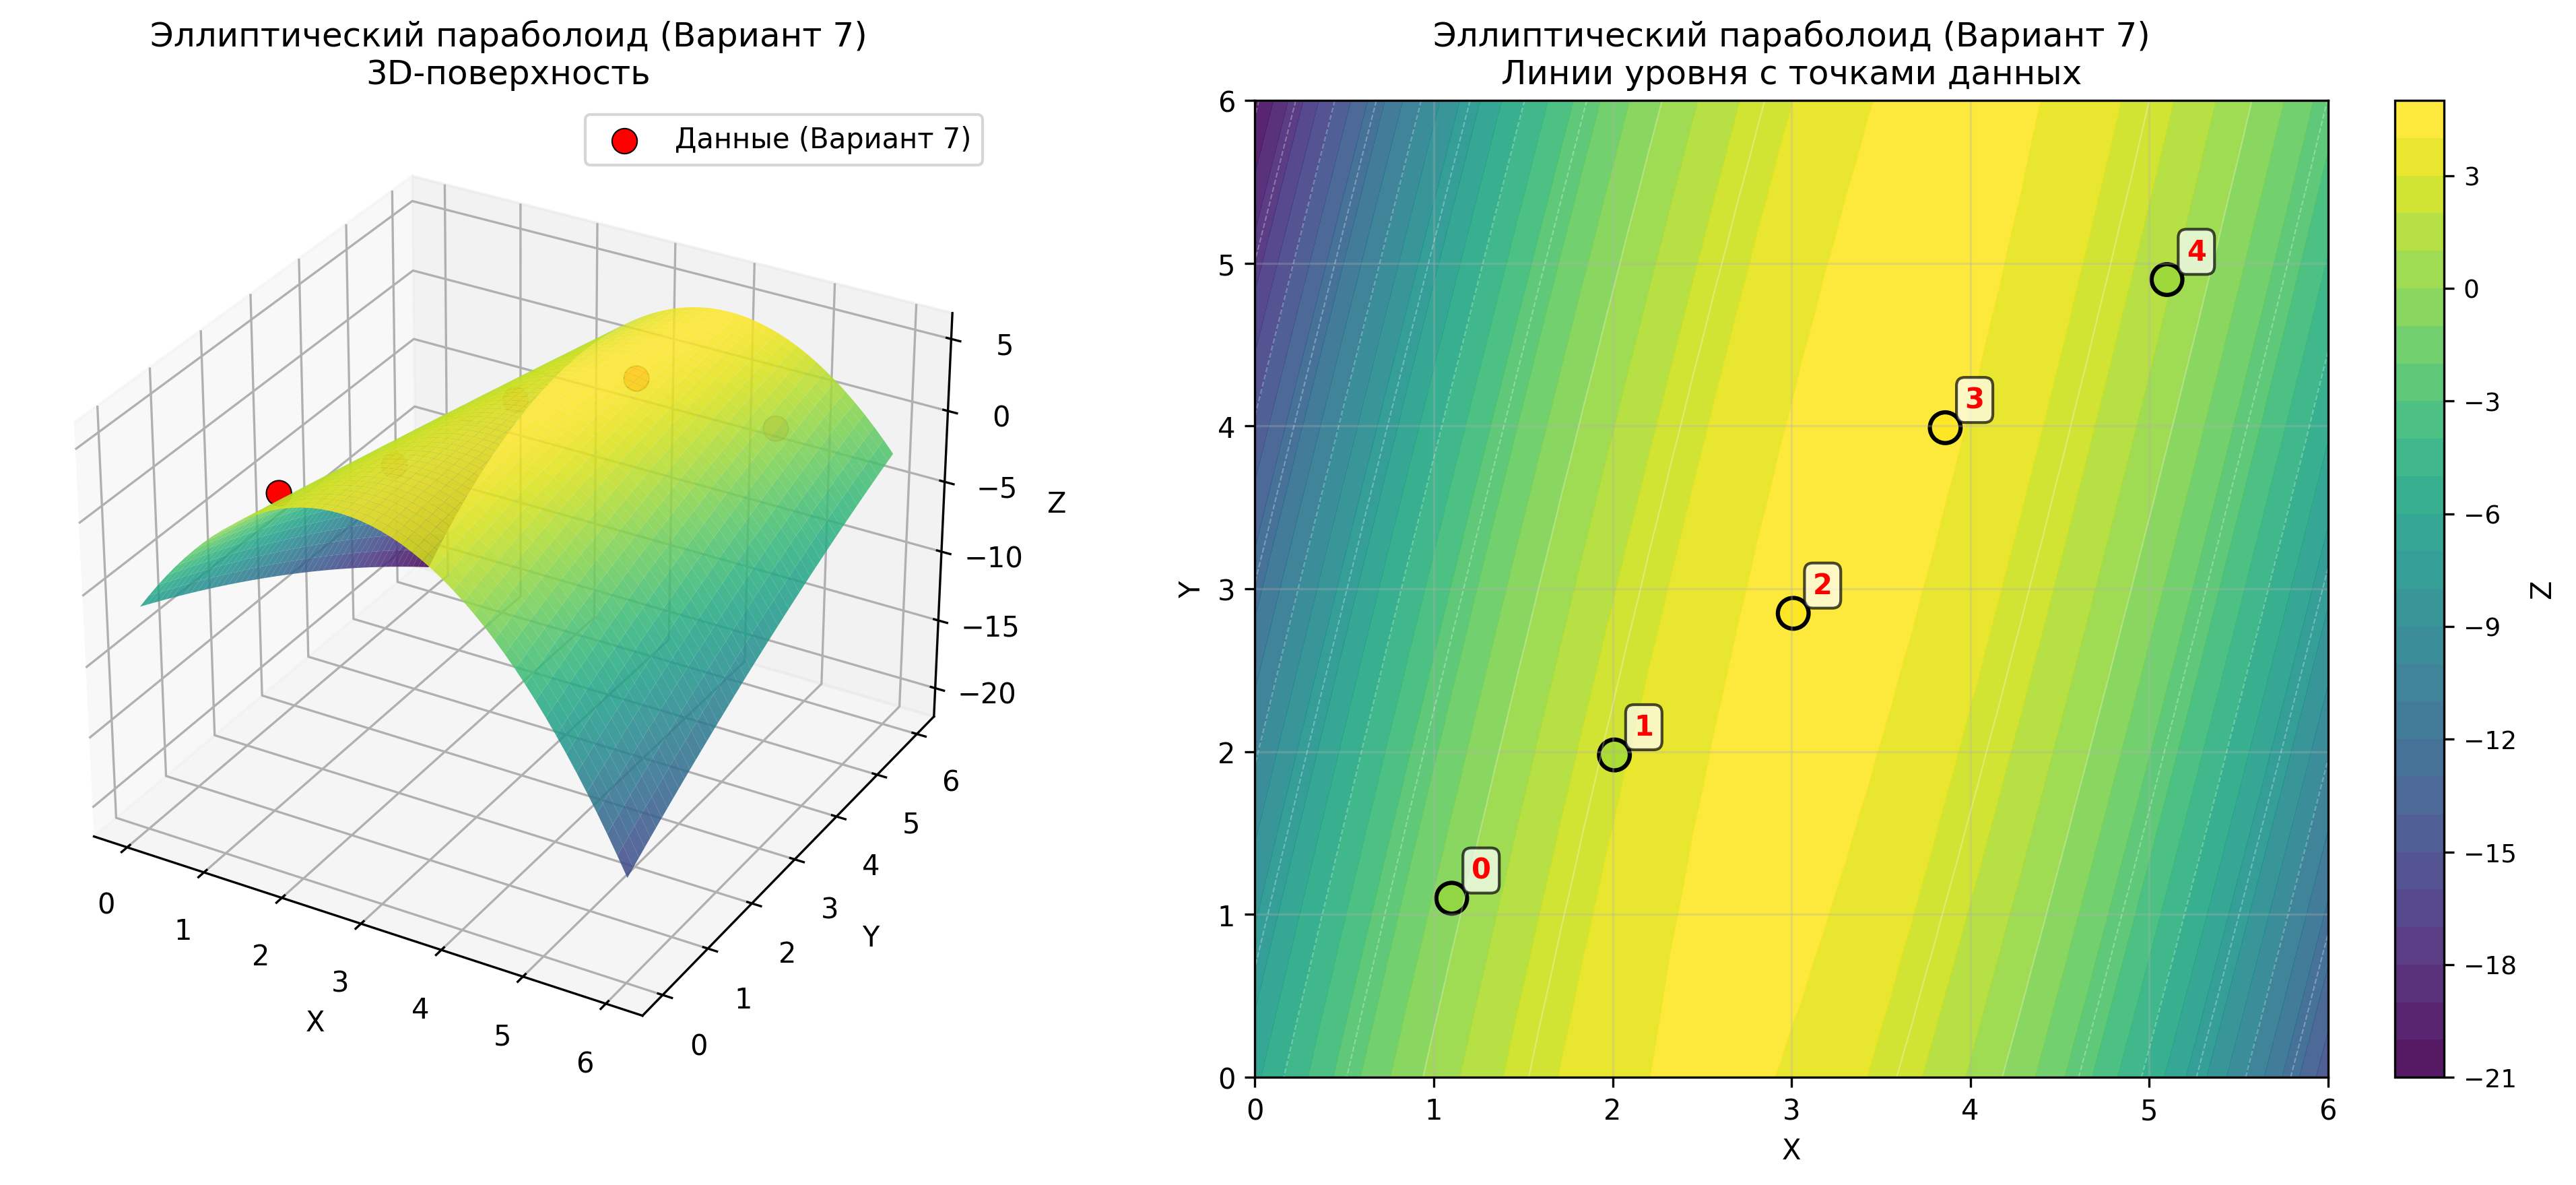
\includegraphics[width=\textwidth]{pic/paraboloid_model.png}
    \caption{Эллиптический параболоид: 3D-поверхность (слева) и линии уровня с точками данных (справа)}
    \label{fig:parab_model}
\end{figure}

Из рис.~\ref{fig:parab_model} видно, что параболическая поверхность не способна описать колоколообразную форму данных. На краях (точки 0 и 4) параболоид даёт значения, далёкие от фактических: в точке 0 модель предсказывает отрицательное значение $-0.38$ вместо $0.29$, а в точке 4 --- $1.15$ вместо $0.77$. Это объясняется тем, что параболоид имеет постоянную кривизну и не может воспроизвести S-образную форму «крыльев» гауссианы.

\subsection{Вывод}

Эллиптический параболоид с 6 параметрами даёт значительные ошибки при аппроксимации данных варианта 7 (MSE = 0.7142). Квадратичная модель принципиально неспособна адекватно описать колоколообразную функцию, поскольку не воспроизводит асимптотическое поведение гауссовых «хвостов». Параболоид следует использовать только для данных, действительно имеющих параболический характер.
